%\subsection{Application performance at higher surge factors}


%The near-optimality of the capacity of all TE schemes is reflected in application performance metrics as well.  Due to sub-optimal capacity of \invcap\ for some TMs, it shows a sub-optimal application performance for these TMs. The relevant graphs are presented in a technical report due to lack of space \cite{TR}. In our analysis, we compare different TE schemes at increasing surge factor for each TM based on application performance metrics - TCP download rate, MOS. We select different percentiles as well as the mean of the distribution of TCP download rate and MOS. As expected, we observe that application performance shows a decline as the surge factor increases towards the SPF value of the TE scheme for a TM. Notably, we do not find any significant difference in application performance of TE schemes irrespective of the statistic we use for comparison. For the TMs where SPF of \invcap\ is sub-optimal, its application performance is worse in comparison to other TE schemes for the same surge factor. 

%
%\begin{figure}[tbh]
%  \begin{center}
%\subfigure[TCP]{\label{fig:TCP_higher_loads}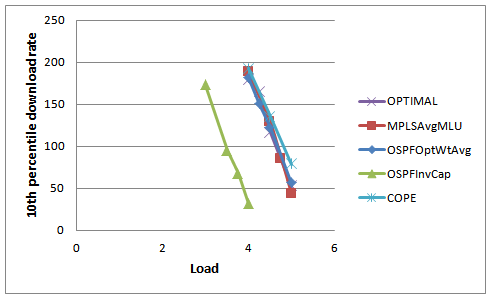
\includegraphics[scale=0.7]{final_images/TCP_higher_loads.png}}
%\subfigure[UDP]{\label{fig:UDP_higher_loads}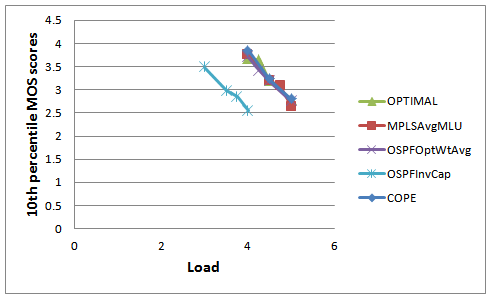
\includegraphics[scale=0.7]{final_images/UDP_higher_loads.png}}
%  \end{center}
%  \caption{TCP and UDP performance at increasing loads for Geant TM}
%\label{fig:higher_loads}
%\end{figure}

% NOTE : Figure moved to previous section

%
%Figure \ref{fig:TCP_higher_loads} shows the 10th percentile of the download throughput distribution at different loads.   All TE schemes have near identical values  except \invcap. The horizontal distance between the curve of \invcap\ and that of other TE schemes curves is approximately equal to the difference in SPF values between them which is indicative of capacity difference between them. Other statistics, e.g. mean, median show similar trends but the horizontal distance between the curve for \invcap\ and other TE schemes reduces at higher percentile values. 

%

%We compute MOS scores for all source-destination pairs as in Section~\ref{sec:UDP_perf}. We find the distribution of MOS scores by selecting node pairs randomly but giving more weight to pairs with more traffic between them. This distribution shows similar trends as the distribution of download throughputs. We do not present the graph due to lack of space. All TE schemes have no significant difference in performance for VoIP traffic based on MOS scores, except \invcap\ which has lower performance at loads near SPF. Note that a VoIP call is a single UDP connection between source and destination nodes without any location diversity, but it still benefits from the rest of the traffic being able to leverage location diversity. 


%We compute MOS scores for source-destination pairs as in Section~\ref{sec:UDP_perf}.  We plot the distribution of MOS scores by selecting node pairs randomly but giving more weight to pairs with more traffic between them. All TE schemes show nearly same performance for VoIP traffic as well. Note that a VoIP call is a singe UDP connection between source and destination nodes without any location diversity, but it still benefits from the rest of the traffic being able to leverage location diversity.


%The curve for UDP shows a similar behavior 

%\textbf{UDP traffic}
%Figure~\ref{fig:UDP_higher_loads}  shows the 10th percentile value of MOS-score distribution at different loads. We compute MOS scores for source-destination pairs as in Section~\ref{sec:UDP_perf}.  We plot the distribution of MOS scores by selecting node pairs randomly but giving more weight to pairs with more traffic between them. All TE schemes show nearly same performance for VoIP traffic as well. Note that a VoIP call is a singe UDP connection between source and destination nodes without any location diversity, but it still benefits from the rest of the traffic being able to leverage location diversity.
